\chapter{Does market power boost profits in Australia?\label{chap:profits}}

Some large firms in Australia are thought to earn high profits by virtue of their market power. As a regulator and a politician put it:

\begin{quote}
    `It is not clear that sustained high profits of the large banks (compared internationally) can be traced to exceptional performance. To the contrary, there appears to be an element that reflects the degree to which the competitors of the large banks are handicapped in their ability to effectively contest the market.'
    
    \rightline{-- \textcite[][1]{ACCC-PC-submission}}
\end{quote}


\begin{quote}
    `Australia’s current regulatory regime has made it too easy for the Coles and Woolworths duopoly to profit at the expense of producers and consumers.'
    
    \rightline{-- Senator Nick \textcite[][219]{Xenophon-minority-report}}
\end{quote}

This chapter assesses these concerns quantitatively right across the non-traded economy.

\section{Profits are higher behind barriers to entry}

\begin{figure}
    \caption{Profits are higher in sectors with barriers to entry \label{fig:ROE-by-barriers}}
    \units{Average return on equity by barriers to entry, per cent}
  \includegraphics[page=18]{atlas/Charts} 
  \notewithsource{Average returns calculated from 2010-11 to 2015-16, weighted by equity, excluding goodwill.}{Grattan analysis of \textcites{IBISWorldIndustry2017}{IBISWorldCompany2017}{Morningstar2017}.}
\end{figure}

Profits are higher in Australia behind barriers to entry. 
\Vref{fig:ROE-by-barriers} shows that high-barrier sectors all earn above-average returns, while low-barrier sectors earn below-average returns: 
\begin{itemize}
    \item \textbf{natural-monopoly} sectors earn an average return on equity of 12 per cent;
    \item \textbf{scale-economy} sectors also earn about 12 per cent;
    \item \textbf{heavy regulation} earn nearly 13 per cent;
    \item \textbf{low barriers} sectors earn a significantly lower average return of about 10 per cent.
\end{itemize}

\newpage

\section{A larger share of profits exceeds the cost of equity behind barriers to entry}

A firm typically seeks to earn profits that exceed the cost of the equity shareholders have invested in it (see \Vref{box:analysis-explained}). 
%Using a standard estimate of the cost of equity , the market cost of equity across Australia was just under 10 per cent over the data period, a little below the average return 
About 20 per cent of the \$200 billion of profits earned across sectors in the non-traded private economy exceeds that estimate cost of equity are in excess of that estimated return required by shareholders. We call them `super-normal' profits. 

\Vref{fig:SNP-pc-of-profit} breaks down the profits within each group of sectors into those earned at or below the cost of equity (`normal' profits, orange), and those earned above the cost of equity (`super-normal' profits, red). 
\begin{itemize}
    \item More than 40 per cent of total profits in natural-monopoly sectors are above the cost of equity;
    \item About 50 per cent of total profits in scale-economy sectors are are above the cost of equity;
    \item Under 20 per cent of total profits earned in the heavily regulated sectors are above the cost of equity, even though that group earns the highest average return on equity;%
    \footnote{That is partly because heavily-regulated sectors are estimated to have higher investment risks.}
    \item Under 20 per cent of total profits earned in the low-barriers sectors exceed the cost of equity. 
\end{itemize}

Overall, about 40 per cent of all super-normal profits are earned behind barriers to entry, even though those sectors account for under 30 per cent of total equity.%
    \footnote{Economists sometimes refer to super-normal profits as `economic profits' or `rents'.}
The other 60 per cent of all super-normal profits are earned in sectors with low barriers to entry, while they account for 70 per cent of total equity. 

\begin{figure}
    \caption{Super-normal profits are higher in sectors with barriers to entry \label{fig:SNP-pc-of-profit}}
    \units{Breakdown of profit by barriers to entry, per cent}
  \includegraphics[page=19]{atlas/Charts} 
  \notewithsource{Excludes traded sectors and those dominated by government firms. Based on average sector returns calculated from 2010-11 to 2015-16.}{Grattan analysis of \textcites{IBISWorldIndustry2017}{IBISWorldCompany2017}{Morningstar2017}.}
\end{figure}

% \Vref{fig:SNP-pc-of-profit} shows that: 
% \begin{itemize}
%     \item In the \textbf{Natural monopoly} sectors, more than 40 per cent of profit is super-profit, or about \$4.5 billion.
%     \item In the \textbf{Scale economy} sectors, more than half of profit is super-profit, or about \$5.8 billion.
%     \item In the \textbf{Heavy regulation} sectors, about 14 per cent of profit is super-profit, or about \$6.4 billion.
%     \item In the \textbf{Low barrier} sectors, about 17 per cent of profit is super-profit, or about \$22 billion.
% \end{itemize}

\newpage

\section{Profits vary a lot across sectors}

Sectors with high barriers to entry earn higher returns on average, but the presence of barriers explains only 7 per cent of the variation in returns.%
    \footnote{Based on the \(R^{2}\) of an equity-weighted regression of sector returns against indicators of barriers to entry.}

Similarly, highly concentrated sectors are more profitable, on average. But concentration explains less than 10 per cent of the variation in returns across sectors.%
    \footnote{Concentrated sectors, by definition, are dominated by a few large firms, and so are more likely to display very high or very low returns.
    For instance, if a dominant firm has an extreme return, this can have a significant impact on the sector-level return, whereas an extreme return from a firm with a small market share will have little impact at the sector level.}
    
\Vref{fig:ROE_conc} shows that there is substantial variation in returns for both high-barrier and low-barrier sectors, regardless of the concentration level.

Returns vary even more widely between individual firms. Operating behind barriers to entry explains only 2 per cent of the variation in average returns over six years at the firm level. Many things affect a firm's returns, including the quality of management and culture, and  innovations in products and processes.

In summary, operating in a concentrated sector with barriers to entry is far from a guarantee of high profitability. But there are a number of sectors behind barriers to entry that are highly profitable, as identified in the following section.
    
\begin{figure}
    \caption{Sector returns are highly variable, especially behind barriers to entry \label{fig:ROE_conc}}
    \units{Return on equity by sector, per cent}
  \includegraphics[page=20]{atlas/Charts} 
  \noteswithsource{Returns are based on averages from 2010-11 to 2015-16. Equity excludes goodwill. Four-firm concentration ratio based on sector revenue. Chart excludes traded sectors and those dominated by government firms. Most sectors are 4-digit ANZSIC, but some have been aggregated to 2-digit ANZSIC due to size or data limitations. Natural monopoly firms are considered to have a 100 per cent concentration ratio in their local market.}{Grattan analysis of \textcites{IBISWorldIndustry2017}{IBISWorldCompany2017}{Morningstar2017}.}
\end{figure}

\begin{bigbox}{Profits, market power and the cost of equity}{box:analysis-explained}

Profit plays an important and legitimate role in society. Protecting and increasing financial value is typically (though not always) prime among an owner's objectives when investing in or running a business.

Profit also plays a critical broader role in the economy by providing signals about what things customers value and how best to produce those things. Profits reward valuable decisions, attract competitors, and direct capital and innovation effort. The owners of firms that get these things right often enjoy a period of high profitability. Customers benefit too, as competing firms make available the things they want most at lower price and in greater volumes and higher quality.

But where profits are high because firms face little competition, they are earned at the expense of customers or suppliers. They are also associated with inefficiencies: the things customers value are curtailed, through high prices, when additional output would be worth more than the cost of the full inputs required to make them available. 
Identifying whether higher profits are due to innovation and cost reduction or to a lack of competitive pressure is difficult. Profitability is influenced by many factors, including innovation effort and risks that can be difficult to measure. A competitive market should, however, ensure that super-normal profits from a given product-set converge towards a normal level over time. Persistently high returns can suggest that competitive pressure is weak, especially if aligned to other measures such as high market concentration and a lack of growth, investment and innovation. 

This chapter uses the return on equity as its profitability measure. That is, the profit (after tax) that a firm reports, for every dollar of shareholders' equity.

The report also uses a concept called the cost of equity. Roughly speaking, that is an estimate of how much return shareholders require. `Normal profit' is earned when the return on equity is equal to the cost of equity. Firms create value for shareholders when their profitability exceeds the cost of equity. `Super-normal' profit (or `economic' profit) is the difference between total profit and normal profit.%
\footnote{When we sum across sectors to yield an estimate of super-normal profit for a group of sectors, we do not provide a discount for sectors that earn below the cost of equity.}

The return on equity at the sector level calculated for this report is the weighted average of firm-level returns over a six-year period. Sector returns are calculated at the 4-digit ANZSIC level, or aggregated to the 2-digit level where firm-level data is too sparse.
%except that very small sectors are aggregated to the 2-digit level where little firm-level data are available, and where it is difficult to distinguish business activity at the 4-digit level.%
Return on equity is adjusted for goodwill to ensure that the profitability measure is not reduced by acquisitions.%
    \footnote{That is, goodwill is subtracted from shareholders' equity -- this is similar to \emph{return on tangible equity}.
    Goodwill represents the amount that a firm has paid above the book value of another firm it has acquired.}

The cost of equity is also estimated for each sector, taking into account a measure of investment risk. Risk is defined using estimates of sector \emph{beta} from the \emph{Capital Asset Pricing Model}.%
    \footnote{Estimates of \emph{beta} are sourced from \textcite{Morningstar2017}. The risk-adjusted cost of equity for each sector is calculated according to the following formula: \(R_{RA(i)} = R_{N} + (\beta_{(i)}-1)R_{RP}\), where \(R_{N}\) is the cost of equity in a sector with an average market level of risk (\(\beta = 1\)), \(\beta_{(i)}\) is the \emph{CAPM beta} for sector \(i\), and \(R_{RP}\) is the market risk premium. This report uses a risk premium of \(6\%\), consistent with \textcite{fernandez2016marketrisk}, and a risk-free rate equal to the average yield on 10-year government bonds from 2011 to 2016, \(3.7\%\); see \textcites{RBA_statistical2017}{RBA_historical2017}. This results in a cost of equity equal to 9.7\(\%\).}
\end{bigbox}

\newpage

% \section{Profitability is somewhat higher in concentrated sectors \label{sec:conc-profits}}

% Sectors with significant barriers to entry are far more likely to be concentrated than those with low barriers to entry (see \Cref{fig:NM_and_Scale} and \Cref{fig:Reg_None}).
% A typical low-barrier sector has a four-firm market share below 20 per cent (with a number of these sectors having no major players), while a typical high-barrier sector has a four-firm market share above 60 per cent.%
%     \footnote{Grattan analysis of \textcite{IBISWorldIndustry2017}.}
% Natural monopoly firms typically have a local market share of 100 per cent in their sector.


% \subsection{High variability in sector-level returns may be explained by high concentration}

% There is an alternative explanation for why returns are more variable in high-barrier sectors.
% It relates to the fact that firm-level returns are highly variable.
% In a sector with many small firms competing, much of the firm-level variability is reduced when returns are aggregated to the sector level.
% But in a concentrated sector, all it takes is for one or two large firms to deviate significantly from the others to skew the sector average well above or below the economy-wide average.

% Given that high-barrier sectors tend to be more concentrated, this statistical phenomenon may explain why the best-performing and worst-performing sectors tend to have barriers to entry.
% It does not mean barriers to entry have no impact on returns, but it does suggest that the presence of high returns in a concentrated sector may not always be due to a lack of competitive pressure.

\section{Some sectors are much more profitable than others, especially behind barriers}

While profitability is highly variable across sectors (\Cref{fig:ROE_conc}), sectors earning profits well above the cost of equity are more prominent behind barriers to entry. This section explores returns for sectors with barriers to entry, and identifies those which are highly profitable.

About 75 percent of sectors behind barriers to entry earn above the cost of equity (when sectors are weighted by the amount of equity). And 20 per cent earn more than 5 percentage points above the cost of equity.
Very high profitability is even more common in natural-monopoly and scale-economy sectors, with half of all equity earning super-normal returns of more than 5 per cent.

Three-quarters of low-barrier sectors also earn above the cost of equity (\Cref{fig:low-barriers} in \Chapref{chap:killer_charts_that_died}).
But very high profitability is far less common, with less than 10 per cent of equity earning super-normal returns of more than 5 per cent. 

\Vref{fig:ROE_barriers} displays the profitability across all sectors with barriers to entry.
The width of each bar denotes shareholder equity, while the height represents the average return on equity.%
    \footnote{Shareholder equity is adjusted to remove goodwill. The most profitable sectors have taller bars, while the largest sectors have wider bars.}
As such, the area of each bar denotes total sector profit.%
    \footnote{This is net profit \emph{after} tax.}

Similarly to \Cref{fig:SNP-pc-of-profit}, sector profit is broken into two components: `normal' profit (orange), and `super-normal' profit (red).%
    \footnote{Sectors earning below the cost of equity do not have a red component. Instead, below-normal profits are shaded grey.}
\Cref{fig:ROE_barriers} is separated into the three barriers-to-entry groups, but the scale is consistent across each.

\begin{figureWhole}
\caption{Sectors with barriers to entry earn more than \$16 billion in super-profits\label{fig:ROE_barriers}}
\units{Average return on equity, per cent} \vspace{2pt} 
\units{Natural-monopoly sectors \hspace{270pt} Sectors with significant scale economies}\vspace{-2pt}
\includegraphics[page=1]{atlas/Barriers.pdf}

\vspace{12pt}

\units{Sectors with heavy regulation}\vspace{-77pt}
\includegraphics[page=2]{atlas/Barriers.pdf}
\noteswithsource{Profits and super-normal profits are \emph{after} tax. Sectors are 4-digit ANZSIC\@. Sector average returns calculated from 2010-11 to 2015-16, weighted by firm equity, excluding goodwill. Shaded areas represent below-normal profits.}{Grattan analysis of \textcites{IBISWorldIndustry2017}{IBISWorldCompany2017}{Morningstar2017}.}
\end{figureWhole}

\subsubsection{Profits in natural-monopoly sectors}

Some natural-monopoly sectors are particularly profitable, as shown in the upper left panel of \Cref{fig:ROE_barriers}.%
    \footnote{Natural-monopoly sectors are typically lower risk, partly reflecting the barriers to entry, and, in some cases, reflecting that returns are regulated in many of these sectors.}

Returns to electricity distribution are nearly double their cost of equity; returns on electricity transmission are lower, but still well above their estimated cost of equity. This may not continue: returns in electricity transmission and distribution are coming down because of tougher regulatory `determinations'.

Returns to the wired telecommunications sector, dominated by Telstra, have been extraordinarily high. This may be due in large part to the fact that most of the copper telecoms network was built long ago, and so its book value is likely to be substantially below its replacement value, while the regulated pricing was determined until recently with reference to an estimate of the full replacement cost of the network.%
\footcite{ACCC2016TelecommunicationsReports}
Looking ahead, the fixed-line telecommunications is progressively shifting to the NBN, radically reshaping the industry. 

Returns to port and water transport terminal operators are, on average, close to the cost of equity, although some port operators are earning substantially higher returns.

Nearly half of returns earned by airport operators are super-normal profits. And some major airports, such as those in Melbourne and Perth, are earning even higher returns.


\newpage

\subsubsection{Profits in scale-economy sectors}

Some scale-economy sectors are earning well above the cost of equity, as shown in the upper right panel of \Cref{fig:ROE_barriers}.

Super-normal profits account for more than half of total profits in supermarkets, liquor retailing, and wireless telecommunications. Returns are even higher for internet service providers and internet publishers, although these sectors are relatively small.

But some sectors with large economies of scale have not delivered high profits, including the four sectors with the lowest returns in the non-traded private economy -- domestic airlines, newspaper publishing, free-to-air TV, and radio broadcasting.

The print and broadcast media were once highly profitable but have struggled against competition from online media. Not coincidentally, the most profitable sector in the non-traded private economy is internet publishing, which includes the profitable and rapidly growing online platforms for employment, housing and car advertisements.

\subsubsection{Profits in sectors with high regulatory barriers}

Sectors with heavier regulation are large, as can be seen from the lower panel of \Cref{fig:ROE_barriers}. The largest, by far, is the banking sector, but general and life insurers are also large relative to other sectors.

Overall, super-normal profits account for only 14 per cent of total profits earned in sectors with heavy regulation, with 80 per cent of these contributed by the banks.
Very high returns are uncommon, with only sports betting and health insurance earning returns more than 5 per cent above their cost of equity.
Banks earn an average return of 14.2 per cent; super-normal profits account for 17 per cent of total profit, once risk is factored in. 

The other highly regulated sectors that earn above-normal profits include residential aged care, pharmacies, taxis, casinos and lotteries. The gambling sectors, although relatively small, earn super-normal profits that may reflect state government licence regulations.%
    \footnote{Our data excludes the non-profit social clubs so does not explicitly pick up revenue from gaming machines.}
The general and life insurance sectors earned a bit below a normal return over the period of the study. 

\subsubsection{Profits in low-barrier sectors}

Sectors with low barriers to entry account for about three-quarters of the non-traded private economy, by value added. Some sectors with low barriers to entry are highly profitable. These are typically a mix of wholesale and retail sectors, professional services, and some construction (\Vref{fig:low-barriers} in \Chapref{chap:killer_charts_that_died}).
But the majority of such sectors earn either a normal return or a relatively small super-normal return.

\section{Profitable firms tend to stay that way, especially behind barriers}

High profits reward innovation and efficiency (\Cref{box:analysis-explained}), but they tend to fade over time. 
Even where firms are able to set high prices for a time, competition tends to wear them down over time:

\begin{quote}
    `If you have faith in open markets, you know that price gouging will often be temporary; that the money being made will attract new entrants and this increase in supply will bring prices down.'
    
    \rightline{-- Rod \textcite{ACCC-role-markets}}
\end{quote}

\begin{figure}
    \caption{Super profits fade about halfway in a decade\label{fig:ROEdecay}}
    \units{Top 200 listed firms by market capitalisation, return on equity, per cent}
  \includegraphics[page=21]{atlas/Charts} 
  \noteswithsource{Median firm within each percentile group. Returns based on 3-year moving average. Top 200 is excluding Exchange-Traded Funds (ETFs), foreign-headquartered firms, mining and metals, and firms with negative equity. Includes firms producing tradeables. Includes ten-year periods beginning 2000 to 2005.}{Grattan analysis of \textcite{Morningstar2017}.}
\end{figure}

\doublecolumnfigure{
{\caption{More than a third of the most profitable firms are still the most profitable ten years later \label{fig:sankey}}
    \units{Return on equity quintiles over ten years, top 200 listed firms by market capitalisation \\ \vspace{2pt} Initial period \hfill After ten years}
  \includegraphics[page=22]{atlas/Charts} 
  \noteswithsource{Returns based on 3-year moving average. Top 200 is excluding Exchange-Traded Funds (ETFs), foreign-headquartered firms, mining and metals, and firms with negative equity. Includes firms producing tradeables. No data in year 10 is either due to firms having missing data or being delisted because they have closed or been acquired.}{Grattan analysis of \textcite{Morningstar2017}.}
}}%
{
\caption{The market expects profits in high-barrier sectors to persist for longer \label{fig:QvsROE}}
    \units{Market-to-book ratio, top 200 listed firms by revenue, 2016}
  \includegraphics[page=23]{atlas/Charts} 
  \noteswithsource{Average return on equity and market-to-book exclude goodwill. Top 200 is excluding Exchange-Traded Funds (ETFs), foreign-headquartered firms, mining and metals, and firms with negative equity. Includes firms producing tradeables. Average return on equity calculated from 2010-11 to 2015-16, with a risk-adjustment using firm-level CAPM \emph{beta}. Average market-to-book by return is estimated using a smooth regression function, and is not equity weighted (applying an equity weight results in an even larger gap between firms from low- and high-barrier sectors). The difference in average market-to-book between high- and low-barrier sectors is significant at the 1\% level, even after controlling for revenue growth over six years.}{Grattan analysis of \textcites{Morningstar2017}{IBISWorldIndustry2017}{IBISWorldCompany2017}.}
}

But it can take many years for high profits to fade toward the cost of equity. Among the 200 largest Australian firms on the ASX (excluding mining), those with high returns initially still over-perform a decade later, by about half as much,  (\Vref{fig:ROEdecay}). The top 10 per cent of firms a decade ago -- earning an average return of 38 per cent -- are typically still earning 22 per cent returns today.%
    \footnote{Returns across firms in the US fade at a similar pace; see \textcite{Koller_ROIC_2010}.}

The most profitable firms are highly likely to remain profitable.
\Vref{fig:sankey} follows the top 200 ASX-listed firms over a decade.%
    \footnote{The analysis includes ten-year periods beginning 2000 to 2005.}
Firms in the top fifth by profitability are more than twice as likely to be there after a decade than less-profitable firms. And firms in the bottom fifth are likely to remain there or drop out completely.%
    \footnote{The `no data' category in \Cref{fig:sankey} represents firms that are either no longer listed, or for which data is missing.}

Profitability persists more strongly for firms in sectors with barriers to entry -- at least, judging by how the market values them.

On average, the market values a firm with recent returns of 20 per cent about 60 per cent higher than a firm with recent returns of 10 per cent.%
    \footnote{If the market expected historical returns to persist indefinitely, it would value the firm with a 20 per cent return at double that of the firm with a 10 per cent return.}
Implicitly, markets expect currently profitable firms to slowly fade towards the average.

But the market expects profits to persist for longer in sectors with barriers to entry.
For a given level of profitability today, investors are prepared to pay a premium of about 20 per cent for shares in firms in protected sectors than for those in sectors where barriers to entry are low (\Vref{fig:QvsROE}). 

\section{Summing up}

Profits are higher behind barriers to entry. Average profitability is about 20 per cent higher in sectors with barriers to entry. And super-normal profits are more likely to be earned behind barriers to entry than in other sectors.
Super-profits in sectors with higher barriers to entry are over \$16 billion a year, or 1 per cent of GDP -- almost as large as the super-normal profits earned in the much bigger group of sectors with low barriers to entry. And markets expect profits behind barriers to stay higher than those elsewhere.

Over \$10 billion of super-normal profit is earned in monopoly sectors or other regulated sectors. That suggests that regulators have not done all they could to ensure consumers get a good deal in these sectors. 

The following chapter explores the implications of market power for consumers -- do they pay more, or do large firms bring down costs so they benefit from scale economies?
